% This file was created with matplot2tikz v0.5.3.
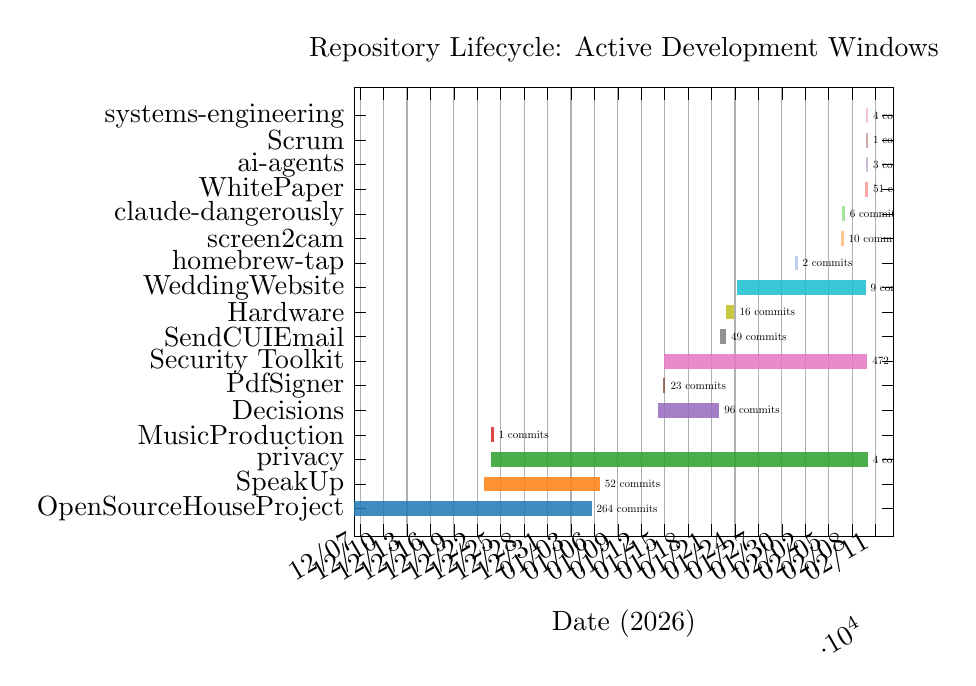
\begin{tikzpicture}

\definecolor{crimson2143940}{RGB}{214,39,40}
\definecolor{darkgray176}{RGB}{176,176,176}
\definecolor{darkorange25512714}{RGB}{255,127,14}
\definecolor{darkturquoise23190207}{RGB}{23,190,207}
\definecolor{forestgreen4416044}{RGB}{44,160,44}
\definecolor{goldenrod18818934}{RGB}{188,189,34}
\definecolor{gray127}{RGB}{127,127,127}
\definecolor{lightgreen152223138}{RGB}{152,223,138}
\definecolor{lightsalmon255152150}{RGB}{255,152,150}
\definecolor{lightsalmon255187120}{RGB}{255,187,120}
\definecolor{lightsteelblue174199232}{RGB}{174,199,232}
\definecolor{mediumpurple148103189}{RGB}{148,103,189}
\definecolor{orchid227119194}{RGB}{227,119,194}
\definecolor{pink247182210}{RGB}{247,182,210}
\definecolor{rosybrown196156148}{RGB}{196,156,148}
\definecolor{sienna1408675}{RGB}{140,86,75}
\definecolor{steelblue31119180}{RGB}{31,119,180}
\definecolor{thistle197176213}{RGB}{197,176,213}

\begin{axis}[
tick pos=both,
title={Repository Lifecycle: Active Development Windows},
x grid style={darkgray176},
xlabel={Date (2026)},
xmajorgrids,
xmin=20428.2232986111, xmax=20497.332171875,
xtick style={color=black},
xtick={20429,20432,20435,20438,20441,20444,20447,20450,20453,20456,20459,20462,20465,20468,20471,20474,20477,20480,20483,20486,20489,20492,20495},
xticklabel style={rotate=30.0,anchor=east},
xticklabels={
  12/07,
  12/10,
  12/13,
  12/16,
  12/19,
  12/22,
  12/25,
  12/28,
  12/31,
  01/03,
  01/06,
  01/09,
  01/12,
  01/15,
  01/18,
  01/21,
  01/24,
  01/27,
  01/30,
  02/02,
  02/05,
  02/08,
  02/11
},
y grid style={darkgray176},
ymin=-1.13, ymax=17.13,
ytick style={color=black},
ytick={0,1,2,3,4,5,6,7,8,9,10,11,12,13,14,15,16},
yticklabels={
  OpenSourceHouseProject,
  SpeakUp,
  privacy,
  MusicProduction,
  Decisions,
  PdfSigner,
  Security Toolkit,
  SendCUIEmail,
  Hardware,
  WeddingWebsite,
  homebrew-tap,
  screen2cam,
  claude-dangerously,
  WhitePaper,
  ai-agents,
  Scrum,
  systems-engineering
}
]
\draw[draw=none,fill=steelblue31119180,fill opacity=0.85] (axis cs:20428.2232986111,-0.3) rectangle (axis cs:20458.6303472222,0.3);
\draw[draw=none,fill=darkorange25512714,fill opacity=0.85] (axis cs:20444.8566319444,0.7) rectangle (axis cs:20459.6861805556,1.3);
\draw[draw=none,fill=forestgreen4416044,fill opacity=0.85] (axis cs:20445.7247569444,1.7) rectangle (axis cs:20494.0001157407,2.3);
\draw[draw=none,fill=crimson2143940,fill opacity=0.85] (axis cs:20445.8004282407,2.7) rectangle (axis cs:20446.1004282407,3.3);
\draw[draw=none,fill=mediumpurple148103189,fill opacity=0.85] (axis cs:20467.0790625,3.7) rectangle (axis cs:20474.9781018519,4.3);
\draw[draw=none,fill=sienna1408675,fill opacity=0.85] (axis cs:20467.7966319444,4.7) rectangle (axis cs:20468.0966319444,5.3);
\draw[draw=none,fill=orchid227119194,fill opacity=0.85] (axis cs:20467.9158680556,5.7) rectangle (axis cs:20493.9470023148,6.3);
\draw[draw=none,fill=gray127,fill opacity=0.85] (axis cs:20475.0858796296,6.7) rectangle (axis cs:20475.8448148148,7.3);
\draw[draw=none,fill=goldenrod18818934,fill opacity=0.85] (axis cs:20475.8720023148,7.7) rectangle (axis cs:20476.9327893519,8.3);
\draw[draw=none,fill=darkturquoise23190207,fill opacity=0.85] (axis cs:20477.2116203704,8.7) rectangle (axis cs:20493.7213773148,9.3);
\draw[draw=none,fill=lightsteelblue174199232,fill opacity=0.85] (axis cs:20484.7094907407,9.7) rectangle (axis cs:20485.0094907407,10.3);
\draw[draw=none,fill=lightsalmon255187120,fill opacity=0.85] (axis cs:20490.5991087963,10.7) rectangle (axis cs:20490.8991087963,11.3);
\draw[draw=none,fill=lightgreen152223138,fill opacity=0.85] (axis cs:20490.7601041667,11.7) rectangle (axis cs:20491.0601041667,12.3);
\draw[draw=none,fill=lightsalmon255152150,fill opacity=0.85] (axis cs:20493.6422916667,12.7) rectangle (axis cs:20494.0355671296,13.3);
\draw[draw=none,fill=thistle197176213,fill opacity=0.85] (axis cs:20493.7296643519,13.7) rectangle (axis cs:20494.0356018519,14.3);
\draw[draw=none,fill=rosybrown196156148,fill opacity=0.85] (axis cs:20493.740474537,14.7) rectangle (axis cs:20494.040474537,15.3);
\draw[draw=none,fill=pink247182210,fill opacity=0.85] (axis cs:20493.7412731481,15.7) rectangle (axis cs:20494.0412731481,16.3);
\draw (axis cs:20458.7803472222,0) node[
  scale=0.4,
  anchor=west,
  text=black,
  rotate=0.0
]{264 commits};
\draw (axis cs:20459.8361805556,1) node[
  scale=0.4,
  anchor=west,
  text=black,
  rotate=0.0
]{52 commits};
\draw (axis cs:20494.1501157407,2) node[
  scale=0.4,
  anchor=west,
  text=black,
  rotate=0.0
]{4 commits};
\draw (axis cs:20446.2504282407,3) node[
  scale=0.4,
  anchor=west,
  text=black,
  rotate=0.0
]{1 commits};
\draw (axis cs:20475.1281018519,4) node[
  scale=0.4,
  anchor=west,
  text=black,
  rotate=0.0
]{96 commits};
\draw (axis cs:20468.2466319444,5) node[
  scale=0.4,
  anchor=west,
  text=black,
  rotate=0.0
]{23 commits};
\draw (axis cs:20494.0970023148,6) node[
  scale=0.4,
  anchor=west,
  text=black,
  rotate=0.0
]{472 commits};
\draw (axis cs:20475.9948148148,7) node[
  scale=0.4,
  anchor=west,
  text=black,
  rotate=0.0
]{49 commits};
\draw (axis cs:20477.0827893519,8) node[
  scale=0.4,
  anchor=west,
  text=black,
  rotate=0.0
]{16 commits};
\draw (axis cs:20493.8713773148,9) node[
  scale=0.4,
  anchor=west,
  text=black,
  rotate=0.0
]{9 commits};
\draw (axis cs:20485.1594907407,10) node[
  scale=0.4,
  anchor=west,
  text=black,
  rotate=0.0
]{2 commits};
\draw (axis cs:20491.0491087963,11) node[
  scale=0.4,
  anchor=west,
  text=black,
  rotate=0.0
]{10 commits};
\draw (axis cs:20491.2101041667,12) node[
  scale=0.4,
  anchor=west,
  text=black,
  rotate=0.0
]{6 commits};
\draw (axis cs:20494.1855671296,13) node[
  scale=0.4,
  anchor=west,
  text=black,
  rotate=0.0
]{51 commits};
\draw (axis cs:20494.1856018519,14) node[
  scale=0.4,
  anchor=west,
  text=black,
  rotate=0.0
]{3 commits};
\draw (axis cs:20494.190474537,15) node[
  scale=0.4,
  anchor=west,
  text=black,
  rotate=0.0
]{1 commits};
\draw (axis cs:20494.1912731481,16) node[
  scale=0.4,
  anchor=west,
  text=black,
  rotate=0.0
]{4 commits};
\end{axis}

\end{tikzpicture}
